% Chapter2


\section{Java}
\subsection{What is Java}
Java is a computing platform and object oriented programming language first released by Sun Microsystems in 1995. Oracle has bought Java in 2010.\cite{JavaWhat}
\\



The Java platform consists of the Java application programming interfaces (APIs) and the Java virtual machine (JVM).
\\



Java is class-bases and object oriented. It is intended to let application developers "write once, run anywhere" meaning that code that runs on one platform does not need to be recompiled to run on another. Java programs are compiled to byte-code. this code can run on any JVM regardless of the real computer architecture.\cite{javaWiki}
\\

Java is next to C/C++ one of the most popular programming languages.\cite{progLangPop} The language also has a similar syntax to C and C++.

\subsection{Class Based \& Object Oriented}
Class-based object-oriented languages, such as Java , are founded on the concept of two distinct entities: classes and instances.\cite{javaObjectClass} 

\begin{enumerate}
\item \textbf{Class:} A class is a blueprint or prototype from which objects are created. \cite{javaOBjectOracle} In class-based languages, you define a class in a separate class definition. In that definition you can specify special methods, called constructors, to create instances of the class. A constructor method can specify initial values for the instance's properties and perform other processing appropriate at creation time.\cite{javaObjectClass} In Java the \textbf{new} Operator is with a call of the constructor method is used to make a new instance of a class. 


\item \textbf{Instance:} An instance or object is the instantiation of a class that is one of its members. Software objects are often used to model the real-world objects

\item \textbf{Interface:} An interface is a collection of empty methods. When a class implements an interface, in java with the keyword \textbf{implements}, it has to implement all methods of the interface. A class describes the attributes and behaviors of an object. An interface contains behaviors that a class implements. 

\item \textbf{Subclasses:} In a class-based language, you create a hierarchy of classes through the class definitions.\cite{javaObjectClass} The subclass, in Java the keyword \textbf{extends} is used, provides all functionalities of the super class an can add new ones ore modify the existing properties.

\begin{figure}[htbp]
\centering
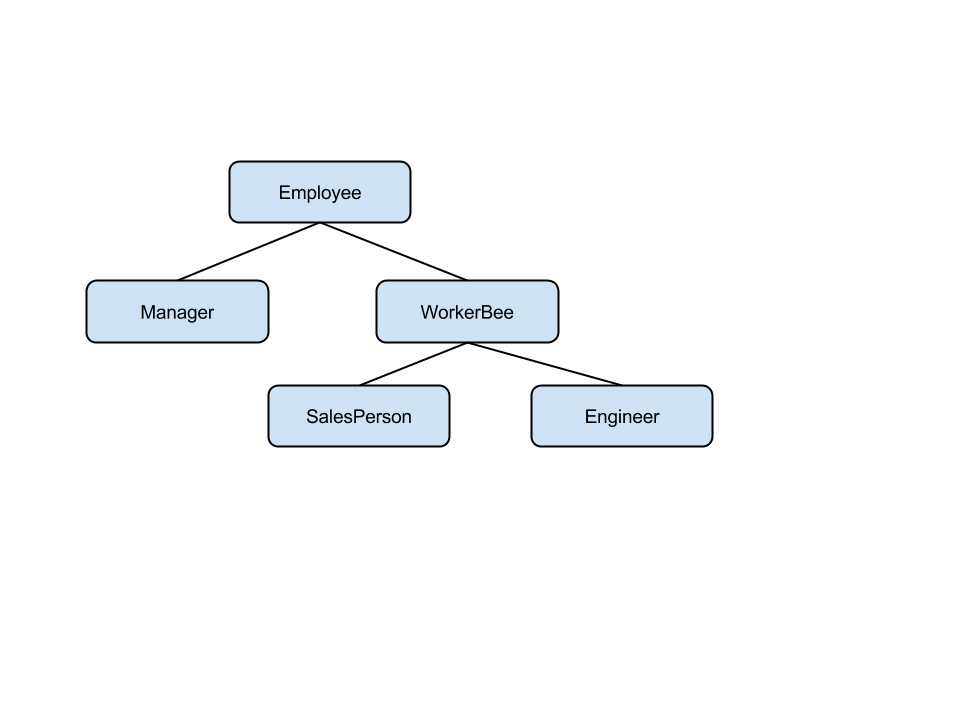
\includegraphics[width=240pt,height=180pt,keepaspectratio]{graphics/java_subclass.png}
\caption{\cite{javaObjectClass}}
\end{figure}
As you can see in this example \textit{Engineer} is an \textit{Employee}. But \textit{Manager} which also is an employee has not the same properties. 


\item \textbf{Abstract Class:}
An abstract class is a class that can't be instantiated. It's only purpose is for other classes to extend. Abstract classes are similar to Interfaces but an abstract class, in contrast, provides more structure. It usually defines some default implementations and provides some tools useful for a full implementation.\cite{javaAbstractVsInterface}

\item \textbf{Package:} 
A package is a namespace for organizing classes and interfaces. Packages make large software projects easier to manage. \cite{javaOBjectOracle}
\end{enumerate}


\subsection{Design Patterns}
Design patterns are proven solutions approaches to specific problems. A design pattern is not a framework! They are based on the base principles of object orientated design. 

\begin{enumerate}
\item Program to an interface not an implementation
\item Favor object composition over inheritance.
\end{enumerate}

\subsection{Performance}
Programs written in Java have the reputation of being slower than other languages. However in the last 10 years the JVM execution speed increased dramatically. In six separate web performance benchmarks, Java frameworks took 22 out of the 24 top-four positions. The JVM has been optimized that much that Java code is now running nearly as fast as C++ code. \cite{javaPerfromance}

\subsection{JVM}
The Java virtual machine is what makes Java a platform independent programming language. A virtual machine (VM) is a software implementation of a machine (i.e. a computer) that executes programs like a physical machine. Therefore, the JVM runs on all kinds of hardware to execute the Java Bytecode without changing the Java execution code. Java developers do not need to know how the JVM exactly works. However a deeper knowledge of the JVM helps understanding how JAVA works and can be helpful to solve various problems.\cite{javaJVM} 
\\


Features of JVM:
\begin{enumerate}
\item \textbf{Stack-based virtual machine:} Most computer architectures such as Intel x86 Architecture and ARM Architecture are based on registers. Whereas the JVM is stack based.\cite{javaJVM} That means that the VM doest need to know the operand addresses, it only calls the Stack-Pointer which points to the current instruction. \cite{stackBased_vs_registerBased} 
\item \textbf{Symbolic reference:} All data types except for primitives are referred to through a symbolic reference.   
\item \textbf{Garbage collection:} The garbage collector frees the memory from objects that are not in use any more. \cite{javaGarbageCollector}  
\item \textbf{Guarantees platform independence by clearly defining the primitive data type:} In other more tradition languages like C or C++ primitive data types have different sizes according to the System. In Java the JVM defines a fixed size for primitives. 
\end{enumerate} \cite{javaJVM}

\subsection{Java bytecode}
The Java bytecode is the result of a compiled Java source-code. It is a middle-language between Java and the machine code. \cite{javaJVM}  

\subsection{Java Code Execution Process} 
The Java code execution process is shown in the following figure. 
\begin{figure}[htbp]
\centering
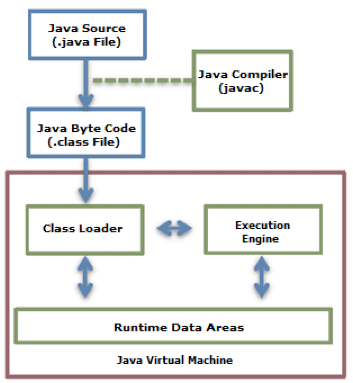
\includegraphics[width=\textwidth,height=\textheight,keepaspectratio]{graphics/java-code-execution-process.png}
\caption{java code execution process \cite{javaJVM}}
\end{figure}
\subsubsection{Class Loader}
The Java Class Loader loads and links a class when it refers to a class the first time at runtime. Every class loader has its own namespace that stores the loaded classes.\cite{javaJVM} 

\subsubsection{Runtime Data Areas}
The JVM Runtime Data Areas is the Memory assigned to a program when it runs on the OS. They can be divided into six areas: the Pc Register, JVM Stack, Native Method Stack, Heap, Method Area, and the Runtime Constant Pool. The first three are created for a single thread the other areas are shared by all threads.  

\begin{enumerate}
\item \textbf{PC register:} One \textbf{program counter} register exists for one thread. It gets created when the thread starts. Pc register has the address of the JVM instruction that is executed now.\cite{javaJVM}
 
\item \textbf{JVM Stack:} Each thread has a private JVM Stack, created the same time as the thread. A Java Virtual Machine stack stores frames. Frames are used to store data and results, new frames are created each time a method is invoked. It gets destroyed when its method invocation completes, whether that completion is normal or abrupt (it throws an uncaught exception). \cite{javaVMOracle}

\item \textbf{Native Method Stack:}
A stack for native code written in a other language than Java. It is a stack used to execute C od C++ Methods.\cite{javaJVM}.  

\item \textbf{Heap:}
The JVM Heap is a data area that is shared among all Java Threads. The heap is created on virtual machine start up.
Its a space that stores all class instances Arrays and Variables. If a program requires more heap space than aviable the Java Virtual Machine throws an \textbf{OutOfMemoryError}\cite{javaVMOracle}

\item. \textbf{Method area:} The method area is shared by all threads, created when the JVM starts. It stores runtime constant pool, field and method information, static variable, and method bytecode for each of the classes and interfaces read by the JVM. Unlike in the heap the garbage collection in the method area is optional for each JVM version. \cite{javaJVM}

\item \textbf{Runtime constant pool:}
The Runtime pool is a part of the Native Method stack and gets created when a class or interface gets created. Its the run-time representation of the \textbf{constant pool} table in a class file. This constant pool table contains several constants \cite{javaVMPaper}

For example:
\begin{lstlisting}[language=Java, caption=Java example Code]
System.out.println("Hello, world!");
\end{lstlisting}
Generated byte-code:
\begin{lstlisting}[language=Java, caption= JVM bytecode]
0:   getstatic       #2;               
3:   ldc     #3;                         
5:   invokevirtual   #4; 
\end{lstlisting}
\#n indicates that this is a reference to the constant pool.
2 is a symbolic reference to \textit{System.out}, \#3 is the \textit{Hello, world!} string.\#4 references to the \textit{PrintStream.println(String)} method.
\cite{javaVmstover}  
\end{enumerate}
\begin{figure}[htbp]
\centering
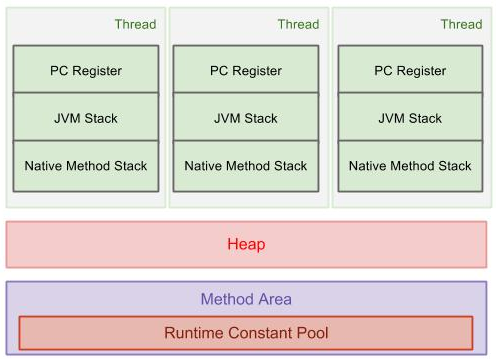
\includegraphics[width=\textwidth,height=\textheight,keepaspectratio]{graphics/java-data-areas.png}
\caption{Java Run-time Data Areas \cite{javaDataAreas}}
\end{figure}
\newpage

\subsubsection{Execution Engine}
The bytecode that is assigned to the runtime data areas in the JVM loaded from the class loader is executed by the execution engine. The execution engine reads the Java Bytecode in the unit of instructions. It is like a real CPU executing the machine commands one by one. Each command consists of 1 Operation Code byte and an additional Operand code. The execution engine gets one OpCode and execute task with the Operand, and then executes the next OpCode.\cite{javaJVM}  

\subsection{.JAR File}
A JAR \textbf{(Java ARchive)}is a file  that contains the class, image, sound, etc. files for a Java application or applet gathered into a single file and possibly compressed. \cite{javaJarMargaret}

\subsubsection{Executable JAR }
Its also possible to create a executable .Jar files. It behaves similar to a .exe file in Windows. It can be executed with a double click when Java is installed on the system. 
